\documentclass{article}
\usepackage{tikz}

\begin{document}

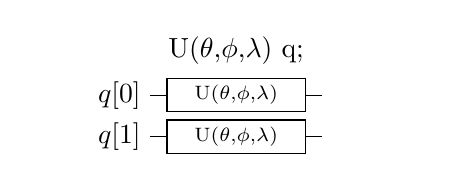
\begin{tikzpicture}[scale=1.000000,x=1pt,y=1pt]
\filldraw[color=white] (0.000000, -7.500000) rectangle (62.000000, 22.500000);
% Drawing wires
% Line 1: q0 W q[0]
\draw[color=black] (0.000000,15.000000) -- (62.000000,15.000000);
\draw[color=black] (0.000000,15.000000) node[left] {$q[0]$};
% Line 2: q1 W q[1]
\draw[color=black] (0.000000,0.000000) -- (62.000000,0.000000);
\draw[color=black] (0.000000,0.000000) node[left] {$q[1]$};
% Done with wires; drawing gates
% Line 3: q0 G {U($\theta$,$\phi$,$\lambda$)} width=50 % U($\theta$,$\phi$,$\lambda$) q;
\draw (31.000000, 22.500000) node[text width=144pt,above,text centered] {U($\theta$,$\phi$,$\lambda$) q;};
\begin{scope}
\draw[fill=white] (31.000000, 15.000000) +(-45.000000:35.355339pt and 8.485281pt) -- +(45.000000:35.355339pt and 8.485281pt) -- +(135.000000:35.355339pt and 8.485281pt) -- +(225.000000:35.355339pt and 8.485281pt) -- cycle;
\clip (31.000000, 15.000000) +(-45.000000:35.355339pt and 8.485281pt) -- +(45.000000:35.355339pt and 8.485281pt) -- +(135.000000:35.355339pt and 8.485281pt) -- +(225.000000:35.355339pt and 8.485281pt) -- cycle;
\draw (31.000000, 15.000000) node {\scriptsize{U($\theta$,$\phi$,$\lambda$)}};
\end{scope}
% Line 4: q1 G {U($\theta$,$\phi$,$\lambda$)} width=50
\begin{scope}
\draw[fill=white] (31.000000, -0.000000) +(-45.000000:35.355339pt and 8.485281pt) -- +(45.000000:35.355339pt and 8.485281pt) -- +(135.000000:35.355339pt and 8.485281pt) -- +(225.000000:35.355339pt and 8.485281pt) -- cycle;
\clip (31.000000, -0.000000) +(-45.000000:35.355339pt and 8.485281pt) -- +(45.000000:35.355339pt and 8.485281pt) -- +(135.000000:35.355339pt and 8.485281pt) -- +(225.000000:35.355339pt and 8.485281pt) -- cycle;
\draw (31.000000, -0.000000) node {\scriptsize{U($\theta$,$\phi$,$\lambda$)}};
\end{scope}
% Done with gates; drawing ending labels
% Done with ending labels; drawing cut lines and comments
% Done with comments
\end{tikzpicture}
\end{document}
